%SECTION%%%%%%%%%%%%%%%%%%%
\section[New Stuff]{4. New and Exciting Stuff}
\begin{frame}
\small{\frametitle{Outline}
\tableofcontents
}
\end{frame}
%%%%%%%%%%%%%%%%%%%%


%% SUBSECTION%%%%%
\subsection[Encoder-Decoder]{Encoder-Decoder Architectures}

%%%
\begin{frame}
\frametitle{So far, we've focused on classification}
\bi
\item Many interesting real-world problems are more complex
\item e.g. Structured prediction, Generation
\item Encoder-Decoders*: a general term for architectures that solve the above 
	\bi
	\item Encodes input $\bf{x}$ (e.g. image) into some representation
	\item Decodes representation to generate structured output $\bf{y}$ (e.g. sentence caption)
	\ei
\ei
\blfootnote{*Not to be confused with auto-encoders}
\end{frame}

%%%
\begin{frame}
\frametitle{Encoder-Decoder explanation (1)}
Recall the recurrent neural net (RNN)\\[0.2cm]
Final hidden state $\bf{c}$ can be used as "encoding" of sequence
\centerline{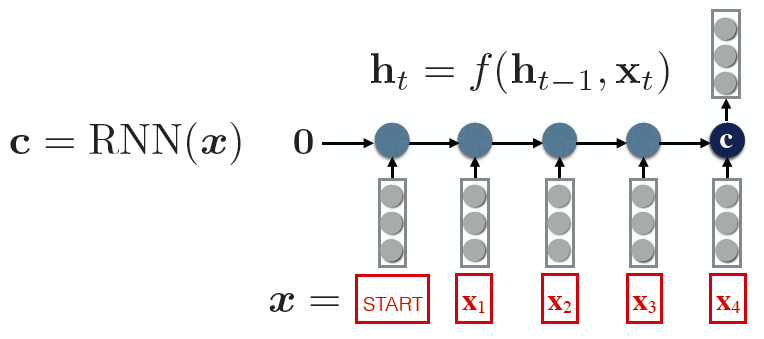
\includegraphics[scale=0.4]{figs/explain_encdec1}}
\end{frame}

%%%
\begin{frame}
\frametitle{Encoder-Decoder explanation (2)}
Recall the recurrent neural net (RNN)\\[0.2cm]
Training objective: predict next word (classification)
\centerline{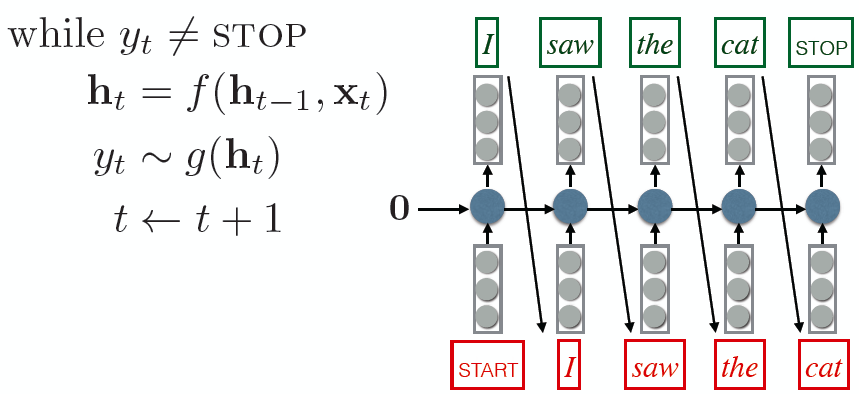
\includegraphics[scale=0.35]{figs/explain_encdec2}}
\end{frame}

%%%
\begin{frame}
\frametitle{Encoder-Decoder explanation (3)}
Simplest Encoder-Decoder: \\[0.2cm]
One RNN for encoding, another RNN for decoding
\bi
\item Decoding can be done by beam search until stop symbol
\item Active research: what is the best encoder or decoder for a specific problem?
\ei
\centerline{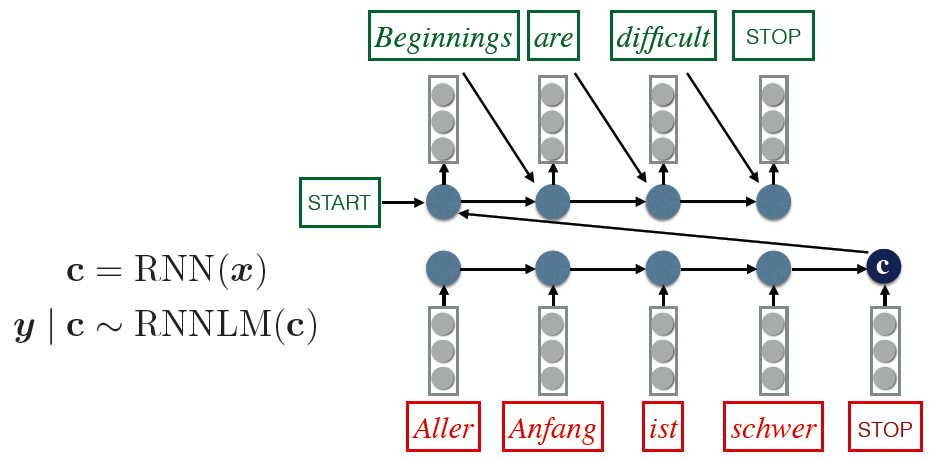
\includegraphics[scale=0.32]{figs/explain_encdec3}}
\end{frame}

%%%
\begin{frame}
\frametitle{Encoder-Decoders for Machine Translation \cite{sutskevar14sequence}}
\begin{scriptsize}("A B C" is source sentence; "W X Y Z" is target sentence)\\Each block is a (deep) LSTM\end{scriptsize}
\centerline{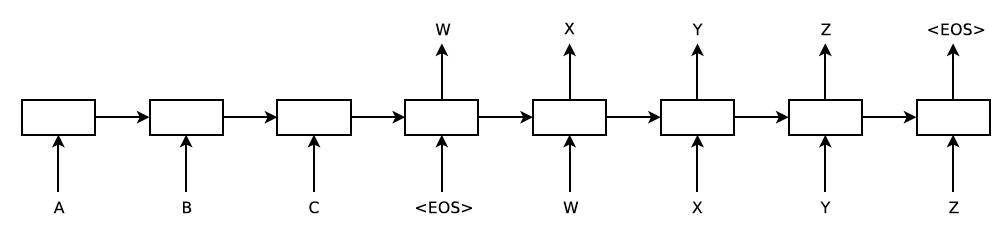
\includegraphics[scale=0.3]{figs/sutskevar14model}}
\bi
\item Training procedure
	\be
	\item Encode source sentence as vector $\bf{c}$
	\item Condition on $\bf{c}$, generate target sentence
	\item Back-prop to optimize target likelihood 
	\ee
\item See \cite{cho14phrase,kalchbrenner13} for other encoder-decoder architecture
\ei
\end{frame}

%%%
\begin{frame}
\frametitle{Encoder-Decoders for Handwriting Generation} 
% TODO: citation, change handwriting example
\centerline{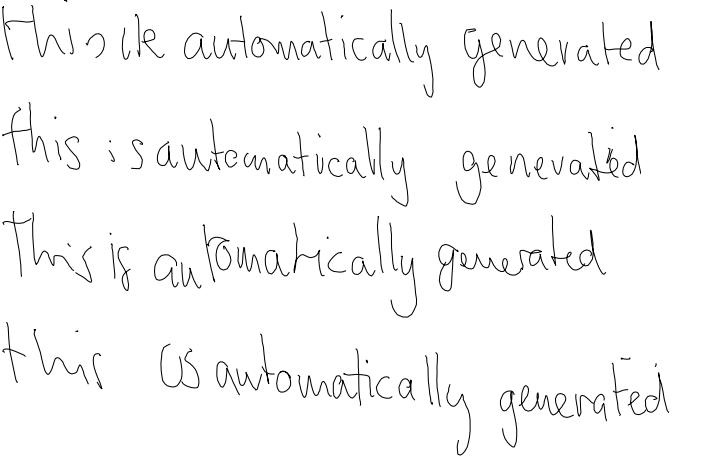
\includegraphics[scale=0.33]{figs/alexgraves_handwriting}}
\url{http://www.cs.toronto.edu/~graves/handwriting.html}
\end{frame}


%% SUBSECTION%%%%%
\subsection[Attention/Memory]{Attention and Memory Mechanism}

%%%
\begin{frame}
\frametitle{Attention: one motivation \cite{bahdanau14translate}}
\bi
\item It seems too much to expect one vector encoding of input $\bf{c}$ can do everything\pause
\item Idea: During decoding, dynamically {\color{red} pay attention} to different parts of the input.
\ei
\pause
\centerline{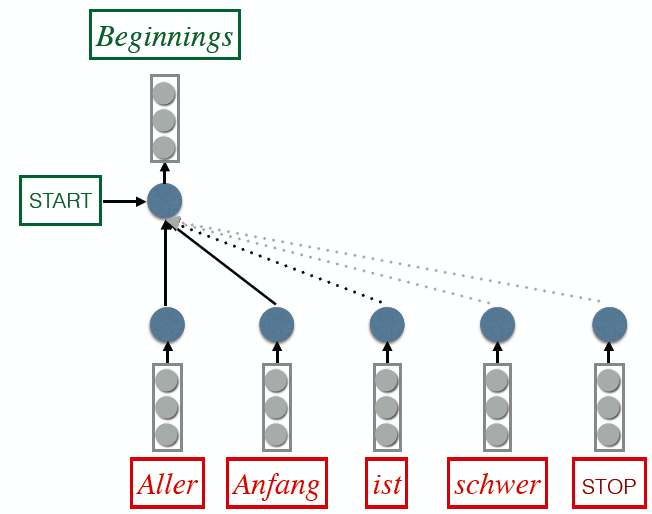
\includegraphics[scale=0.33]{figs/explain_attention1}}
\end{frame}

%%%
\begin{frame}
\frametitle{Attention: one motivation \cite{bahdanau14translate}}
\bi
\item It seems too much to expect one vector encoding of input $\bf{c}$ can do everything
\item Idea: During decoding, dynamically {\color{red} pay attention} to different parts of the input.
\ei
\centerline{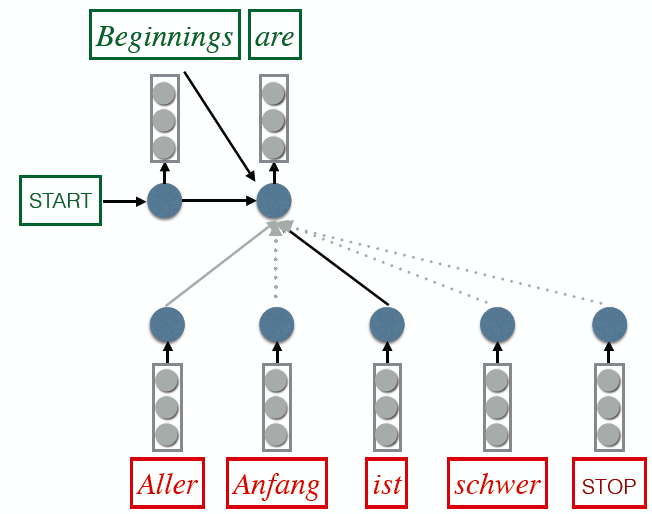
\includegraphics[scale=0.33]{figs/explain_attention2}}
\end{frame}

%%%
\begin{frame}
\frametitle{Attention: one motivation \cite{bahdanau14translate}}
\bi
\item It seems too much to expect one vector encoding of input $\bf{c}$ can do everything
\item Idea: During decoding, dynamically {\color{red} pay attention} to different parts of the input.
\ei
\centerline{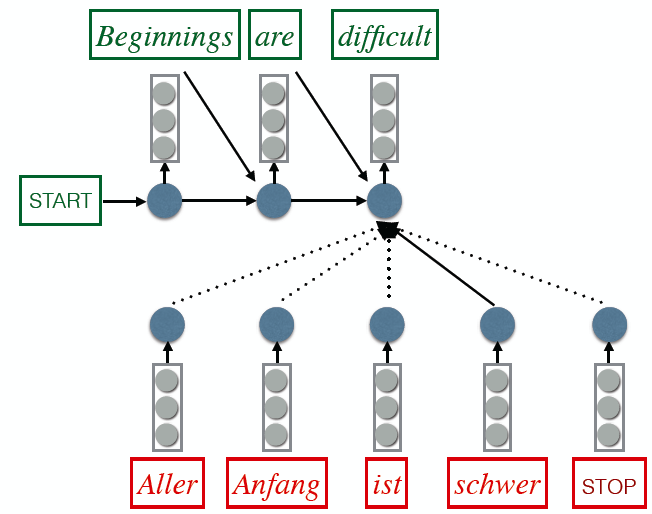
\includegraphics[scale=0.33]{figs/explain_attention3}}
\end{frame}

%%%
\begin{frame}
\frametitle{Attention: one motivation \cite{bahdanau14translate}}
\bi
\item It seems too much to expect one vector encoding of input $\bf{c}$ can do everything
\item Idea: During decoding, dynamically {\color{red} pay attention} to different parts of the input.
\ei
\centerline{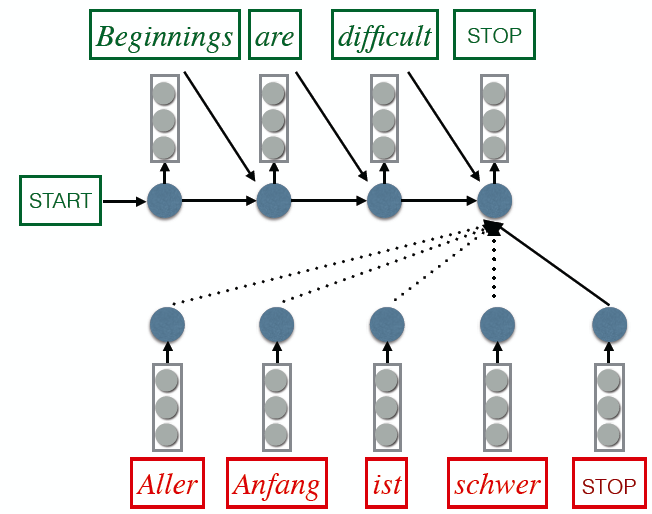
\includegraphics[scale=0.33]{figs/explain_attention4}}
\end{frame}

%%%
\begin{frame}
\frametitle{Encoder-Decoders with Attention}
Caption Generation \cite{xu15caption}: 
\bi
\item Input = image, Output = sentence caption
\item Attention = image patch
\ei
\centerline{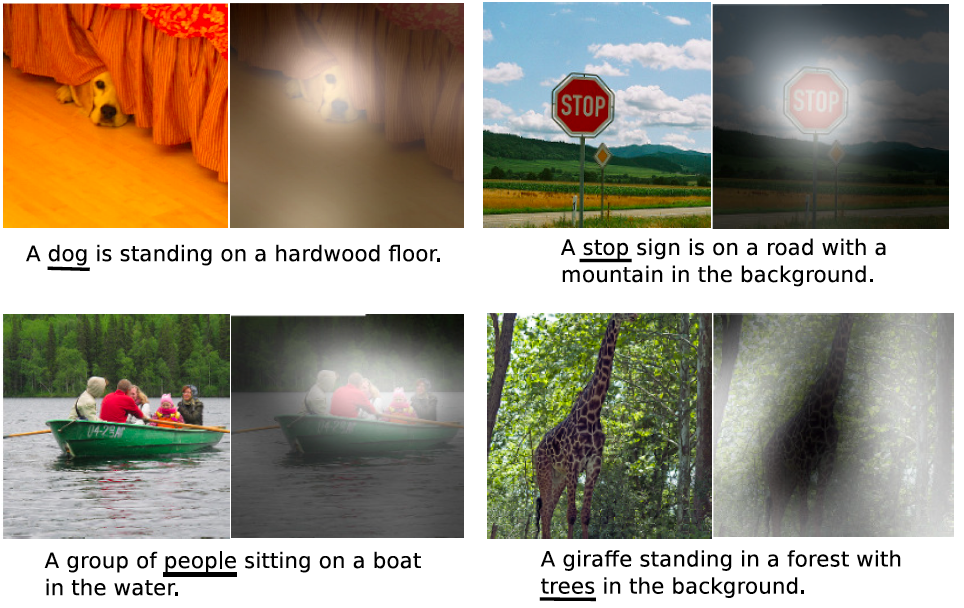
\includegraphics[scale=0.3]{figs/xu15_example}}
\end{frame}

%%%
\begin{frame}
\frametitle{Encoder-Decoders with Attention}
Caption Generation \cite{xu15caption}:
\bi
\item Input = image, Output = sentence caption
\item Attention = image patch
\ei
\centerline{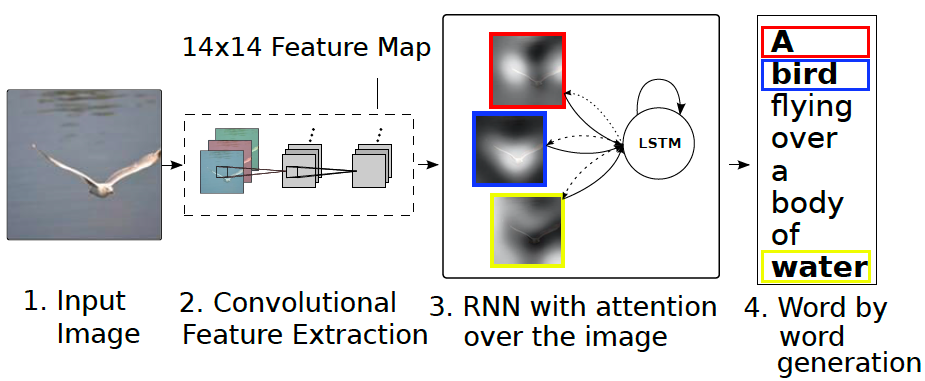
\includegraphics[scale=0.3]{figs/xu15_model}}
\end{frame}

%%%
\begin{frame}
\frametitle{Encoder-Decoders with Attention}
Abstractive Sentence Summarization \cite{rush15abstractive}:
\bi
\item Input = Long sentence, Output = Short sentence
\item Attention = words
\ei
\centerline{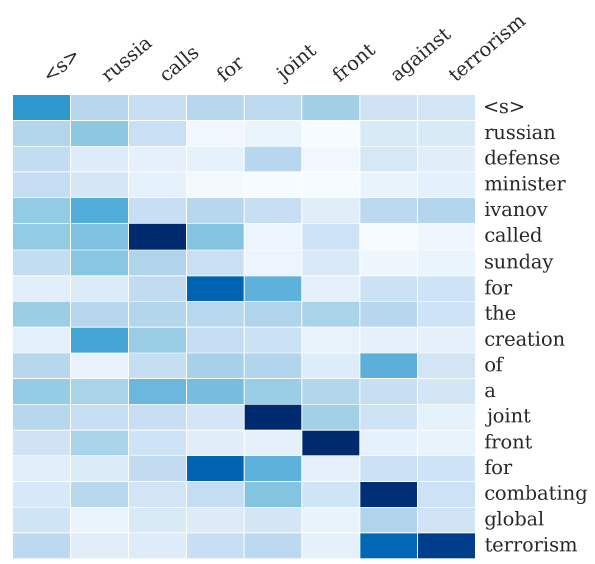
\includegraphics[scale=0.33]{figs/rush15_example}}
\end{frame}

%%%
\begin{frame}
\frametitle{Attention, Memory, and Neural Turing Machines}
\bi
\pause
\item Let's ponder about human learning: \pause
\bi
	\item You can't learn if you don't pay attention \pause
	\item Need to keep relevant concepts in working memory to build up new concepts \pause
\ei
\item Active research: Finding new architectures (preferably differentiable) that allows this kind of learning \cite{graves14turing,weston14memory}
\ei 
\centerline{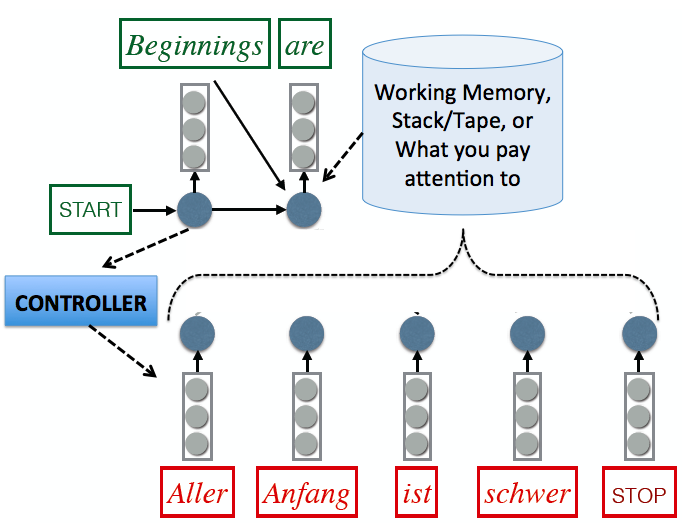
\includegraphics[scale=0.27]{figs/attention_memory_stack}}
\end{frame}


%% SUBSECTION%%%%%
\subsection[Deep Reinforcement]{Deep Reinforcement Learning}

%%%
\begin{frame}
\frametitle{Reinforcement Learning}
\bi
\item Reinforcement Learning can be viewed as general-purpose tool for AI
\bi
	\item We have an {\color{red} agent} with ability to {\color{red} act}
	\item Each {\color{red} action} affects future {\color{red} state}
	\item Plan a set of actions to maximize final {\color{red} reward}
\ei
\pause
\item Policy $\pi$: selects actions given states $a=\pi(s)$
\item Value function $Q^\pi(s,a) = E_\pi[r_{t+1}+\eta r_{t+2} + \eta^2 r_{t+3} \cdots | s,a]$: expected future reward from ($s,a$) under $\pi$ 
\item Optimal Value function $Q^\pi(s,a) = E_\pi[r_{t+1}+\eta r_{t+2} + \eta^2 r_{t+3} \cdots | s,a]$: expected future reward from ($s,a$) under any policy.
\ei
\end{frame}

%%%
\begin{frame}
\frametitle{Deep Reinforcement Learning (Q-learning approach)}
\bi 
\item Estimate value function by neural net: $Q(s,a;w) \approx Q^\pi(s,a)$
\item Training objective: mean square error of Q-values: 
\begin{math}
L(w)=E[\left(y - Q(s,a;w)\right)^2]
\end{math}\\[0.2cm]
where $y= E[r+\eta \max_{a'} Q(s',a'; w_{previous}) | s,a] $ is optimal value under previous weights
\item Train by playing out the actions. See \cite{mnih13atari} for important tricks to get it working
\ei
\end{frame}

%%%
\begin{frame}
\frametitle{Deep Reinforcement Learning for Playing Atari \cite{mnih13atari}}
\centerline{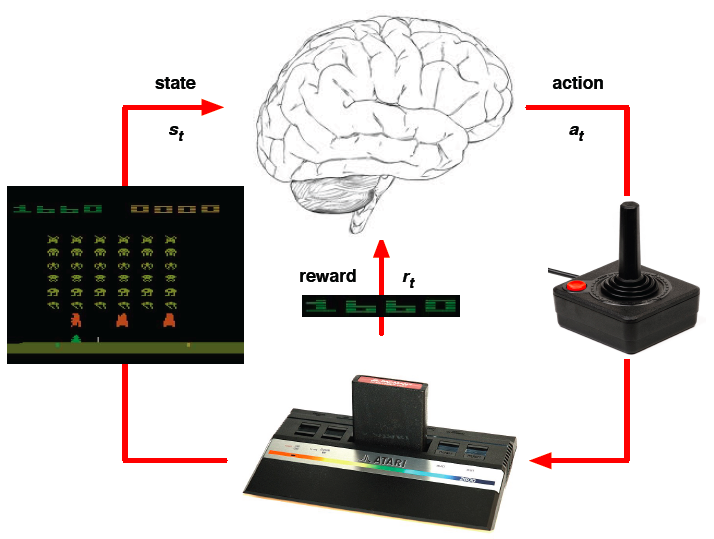
\includegraphics[scale=0.4]{figs/dqn_atari}}
\small{Figure from D. Silver's ICLR2015 keynote slides}
\end{frame}


%% SUBSECTION%%%%%
\subsection[Variational Auto-Encoder]{Auto-Encoding Variational Bayes}

%%%%%%
\begin{frame}
\frametitle{Motivation: Directed Probabilistic Models}
\bi
\item How to perform learning and inference on directed probabilistic models, in the presence of continuous latent variables with intractable posteriors? \pause
\item Generative process:
	\be
	\item Draw continuous latent variable $\bf{z}$ $\sim$ prior $p_{\theta^*}(\bf{z})$ 
	\item Draw data $\bf{x}$ $\sim$ $p_{\theta^*}(\bf{x}|\bf{z})$ 
	\ee 
	\bi
	\item True $\bf{z}$ for each data and parameter $\theta^*$ are unknown
	\ei
	\centerline{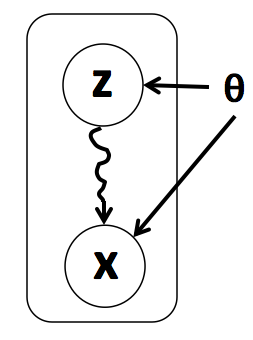
\includegraphics[scale=0.2]{figs/autoencoding_variationalbayes1}}
	\pause
\item Assume marginal likelihood $p_{\theta}(\bf{x})$ and posterior $p_{\theta}(\bf{z}|\bf{x})$ are intractable. Can't differentiate likelihood. Can't do EM.
\ei

\end{frame}

%%%
\begin{frame}
\frametitle{Autoencoding Variational Bayes \cite{kingma14variational}}
\bi
\item Idea: Introduce {\color{red} recognition model} $p_{\phi}(\bf{z}|\bf{x})$ as approximation to posterior $p_{\theta}(\bf{z}|\bf{x})$. 
\item Unlike mean-field variational inference, it's not factorial \& parameters need not be computed in closed-form.\pause
\item Reparameterize ${\bf{\hat{z}}} \sim p_{\phi}(\bf{z}|\bf{x})$ as ${\bf{\hat{z}}} = g_{\phi}(\bf{x}, \epsilon)$
	\bi
	\item $g_\phi()$ is non-linear transform, e.g. MLP
	\item $\epsilon$ is drawn from noise distribution
	\item Using this, one can take derivative of VB bound!\pause
	\ei
\item Implications:
\bi
	\item Training deep generative models on large data
	\item Semi-supervised learning \cite{kingma14ssl}
\ei
\ei
\end{frame}


%%%%%%
\begin{frame}
\frametitle{Section Summary}
\bi
\item Encoder-Decoder Architectures
\item Attention and Memory Mechanism
\item Deep Reinforcement Learning
\item Auto-Encoding Variational Bayes
\ei 
\end{frame}



